% ==============================================================================
\chapter{Discretization: Isogeometric Analysis (IGA)}
\label{ch:discretization}
% ==============================================================================

\begin{tcolorbox}[colback=lightbg, colframe=primaryblue, title=\textbf{Chapter at a Glance: CAD-Integrated Discretization}, fonttitle=\bfseries]
    \begin{description}[leftmargin=!, labelwidth=3.4cm]
        \item[\textbf{Core Paradigm}] Use Non-Uniform Rational B-Splines (NURBS) as basis functions for both geometry definition and elastodynamic state approximation.
        \item[\textbf{Refinement Vectors}] $h$-refinement (knot insertion), $p$-refinement (degree elevation), and $k$-refinement (order elevation maintaining $C^{p-1}$ continuity).
        \item[\textbf{System Output}] Semi-discrete matrix equations of motion $\mat{M}\ddot{\vect{d}} + \mat{C}\dot{\vect{d}} + \mat{K}\vect{d} = \vect{F}_{\text{ext}}$ without geometry discretization error.
    \end{description}
\end{tcolorbox}

Following the continuum elastodynamic formulation established in Chapter \ref{ch:theory}, discretizing the governing equations requires a spatial basis capable of handling complex geometry accurately. Traditional finite element methods introduce geometric approximation errors when tessellating curved boundaries into polygonal meshes. This chapter develops Isogeometric Analysis (IGA), which employs Non-Uniform Rational B-Splines (NURBS) as basis functions for both geometry definition and elastodynamic state approximation, producing exact CAD boundary representation and continuous semi-discrete equations of motion.

% ------------------------------------------------------------------------------
\section{B-Splines \& NURBS Geometry Representation}
% ------------------------------------------------------------------------------

Here, we introduce univariate B-splines, rational NURBS basis functions, and tensor-product surface patches that form the foundation of IGA.

Isogeometric Analysis (IGA), pioneered by Hughes et al. \cite{hughes2005} and expanded by Cottrell et al. \cite{cottrell2009}, eliminates the gap between Computer-Aided Design (CAD) and Finite Element Analysis (FEA) by employing NURBS basis functions directly in the analysis solver.

\subsection{Univariate B-Spline Basis \& Cox-de Boor Recurrence}
Cox-de Boor recurrence relations and derivative formulas for univariate B-spline basis functions are defined as follows.

Given an open knot vector $\Xi = \{\xi_0, \xi_1, \dots, \xi_m\}$, univariate B-spline basis functions $N_{i,p}(\xi)$ of degree $p$ are defined recursively via the Cox-de Boor formula:

\begin{equation}
    N_{i,0}(\xi) = \begin{cases} 1 & \text{if } \xi_i \le \xi < \xi_{i+1} \\ 0 & \text{otherwise} \end{cases}
\end{equation}
\begin{equation}
    N_{i,p}(\xi) = \frac{\xi - \xi_i}{\xi_{i+p} - \xi_i} N_{i,p-1}(\xi) + \frac{\xi_{i+p+1} - \xi}{\xi_{i+p+1} - \xi_{i+1}} N_{i+1,p-1}(\xi)
\end{equation}

Analytical spatial gradients for strain evaluations are computed using derivative recurrence:
\begin{equation}
    \frac{d}{d\xi} N_{i,p}(\xi) = p \left( \frac{N_{i,p-1}(\xi)}{\xi_{i+p} - \xi_i} - \frac{N_{i+1,p-1}(\xi)}{\xi_{i+p+1} - \xi_{i+1}} \right)
\end{equation}
Evaluating quadratic B-spline basis functions $N_{i,2}(\xi)$ over an open knot vector yields smooth localized shape functions with partition of unity properties (Figure \ref{fig:nurbs_curves_eval}).

\begin{figure}[htbp]
    \centering
    \makebox[\textwidth][c]{%
        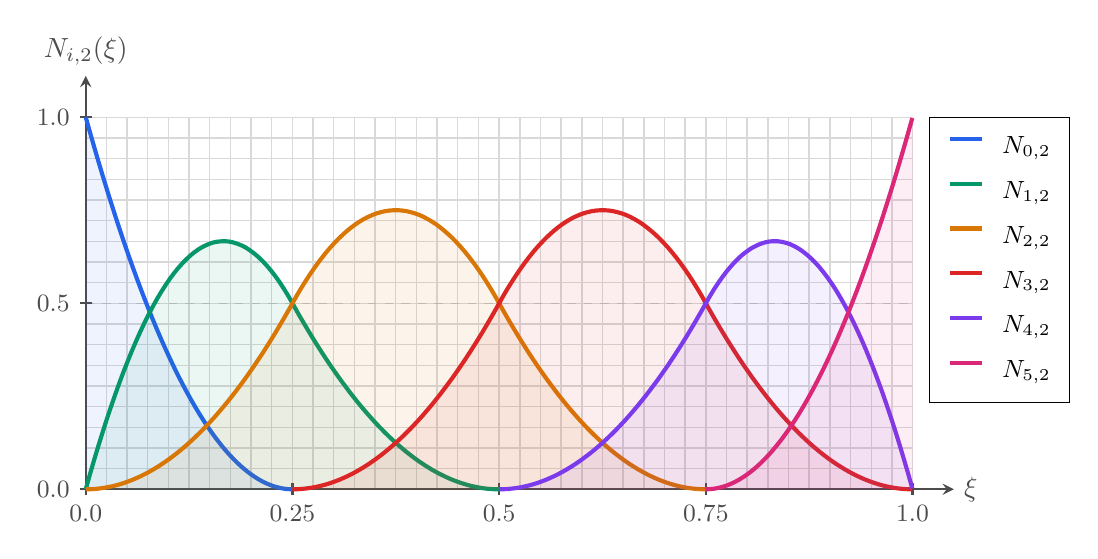
\begin{tikzpicture}[scale=1.05, >=stealth]
            \definecolor{n0color}{RGB}{37, 99, 235}
            \definecolor{n1color}{RGB}{5, 150, 105}
            \definecolor{n2color}{RGB}{217, 119, 6}
            \definecolor{n3color}{RGB}{220, 38, 38}
            \definecolor{n4color}{RGB}{124, 58, 237}
            \definecolor{n5color}{RGB}{219, 39, 119}

            \draw[gray!30, line width=0.5pt] (0, 0) grid[ystep=0.25, xstep=0.25] (10, 4.5);
            \draw[gray!50, dashed, line width=0.5pt] (0, 2.25) -- (10, 2.25);

            \draw[->, thick, black!70] (0,0) -- (10.5,0) node[right] {$\xi$};
            \draw[->, thick, black!70] (0,0) -- (0,5.0) node[above] {$N_{i,2}(\xi)$};

            \foreach \x/\label in {0/0.0, 2.5/0.25, 5/0.5, 7.5/0.75, 10/1.0} {
                    \draw[black!70, thick] (\x, 2pt) -- (\x, -2pt) node[below, font=\small] {\label};
                }
            \foreach \y/\label in {0/0.0, 2.25/0.5, 4.5/1.0} {
                    \draw[black!70, thick] (2pt, \y) -- (-2pt, \y) node[left, font=\small] {\label};
                }

            \fill[n0color, opacity=0.08] (0,4.5) -- plot[domain=0:0.25, samples=50] ({10*\x}, {4.5*(1-4*\x)^2}) -- (2.5,0) -- (0,0) -- cycle;
            \draw[n0color, line width=1.5pt] plot[domain=0:0.25, samples=50] ({10*\x}, {4.5*(1-4*\x)^2});

            \fill[n1color, opacity=0.08] (0,0) -- plot[domain=0:0.25, samples=50] ({10*\x}, {4.5*(8*\x - 24*\x^2)}) -- plot[domain=0.25:0.5, samples=50] ({10*\x}, {4.5*(8*(0.5-\x)^2)}) -- (5,0) -- cycle;
            \draw[n1color, line width=1.5pt] plot[domain=0:0.25, samples=50] ({10*\x}, {4.5*(8*\x - 24*\x^2)}) -- plot[domain=0.25:0.5, samples=50] ({10*\x}, {4.5*(8*(0.5-\x)^2)});

            \fill[n2color, opacity=0.08] (0,0) -- plot[domain=0:0.25, samples=50] ({10*\x}, {4.5*(8*\x^2)}) -- plot[domain=0.25:0.5, samples=50] ({10*\x}, {4.5*(12*\x - 16*\x^2 - 1.5)}) -- plot[domain=0.5:0.75, samples=50] ({10*\x}, {4.5*(8*(0.75-\x)^2)}) -- (7.5,0) -- cycle;
            \draw[n2color, line width=1.5pt] plot[domain=0:0.25, samples=50] ({10*\x}, {4.5*(8*\x^2)}) -- plot[domain=0.25:0.5, samples=50] ({10*\x}, {4.5*(12*\x - 16*\x^2 - 1.5)}) -- plot[domain=0.5:0.75, samples=50] ({10*\x}, {4.5*(8*(0.75-\x)^2)});

            \fill[n3color, opacity=0.08] (2.5,0) -- plot[domain=0.25:0.5, samples=50] ({10*\x}, {4.5*(8*(\x-0.25)^2)}) -- plot[domain=0.5:0.75, samples=50] ({10*\x}, {4.5*(12*(1-\x) - 16*(1-\x)^2 - 1.5)}) -- plot[domain=0.75:1.0, samples=50] ({10*\x}, {4.5*(8*(1-\x)^2)}) -- (10,0) -- cycle;
            \draw[n3color, line width=1.5pt] plot[domain=0.25:0.5, samples=50] ({10*\x}, {4.5*(8*(\x-0.25)^2)}) -- plot[domain=0.5:0.75, samples=50] ({10*\x}, {4.5*(12*(1-\x) - 16*(1-\x)^2 - 1.5)}) -- plot[domain=0.75:1.0, samples=50] ({10*\x}, {4.5*(8*(1-\x)^2)});

            \fill[n4color, opacity=0.08] (5,0) -- plot[domain=0.5:0.75, samples=50] ({10*\x}, {4.5*(8*(\x-0.5)^2)}) -- plot[domain=0.75:1.0, samples=50] ({10*\x}, {4.5*(8*(1-\x) - 24*(1-\x)^2)}) -- (10,0) -- cycle;
            \draw[n4color, line width=1.5pt] plot[domain=0.5:0.75, samples=50] ({10*\x}, {4.5*(8*(\x-0.5)^2)}) -- plot[domain=0.75:1.0, samples=50] ({10*\x}, {4.5*(8*(1-\x) - 24*(1-\x)^2)});

            \fill[n5color, opacity=0.08] (7.5,0) -- plot[domain=0.75:1.0, samples=50] ({10*\x}, {4.5*(4*\x-3)^2}) -- (10,4.5) -- (10,0) -- cycle;
            \draw[n5color, line width=1.5pt] plot[domain=0.75:1.0, samples=50] ({10*\x}, {4.5*(4*\x-3)^2});

            \matrix [draw, fill=white, at={(10.2, 4.5)}, anchor=north west, font=\small, row sep=1pt, ampersand replacement=\&] {
                \node {\tikz[baseline=-0.5ex]{\draw[n0color, line width=1.5pt] (0,0) -- (0.4,0);}}; \& \node {$N_{0,2}$}; \\
                \node {\tikz[baseline=-0.5ex]{\draw[n1color, line width=1.5pt] (0,0) -- (0.4,0);}}; \& \node {$N_{1,2}$}; \\
                \node {\tikz[baseline=-0.5ex]{\draw[n2color, line width=1.5pt] (0,0) -- (0.4,0);}}; \& \node {$N_{2,2}$}; \\
                \node {\tikz[baseline=-0.5ex]{\draw[n3color, line width=1.5pt] (0,0) -- (0.4,0);}}; \& \node {$N_{3,2}$}; \\
                \node {\tikz[baseline=-0.5ex]{\draw[n4color, line width=1.5pt] (0,0) -- (0.4,0);}}; \& \node {$N_{4,2}$}; \\
                \node {\tikz[baseline=-0.5ex]{\draw[n5color, line width=1.5pt] (0,0) -- (0.4,0);}}; \& \node {$N_{5,2}$}; \\
            };
        \end{tikzpicture}%
    }
    \caption{Quadratic B-spline basis functions $N_{i,2}(\xi)$ evaluated over knot vector $\Xi = \{0, 0, 0, 0.25, 0.5, 0.75, 1, 1, 1\}$.}
    \label{fig:nurbs_curves_eval}
\end{figure}

\subsection{Non-Uniform Rational B-Splines (NURBS)}
Rational basis functions with projective weights are formulated to represent exact conic and curved geometries.

Projective control weights $w_i$ define the rational basis functions $R_{i,p}(\xi)$:
\begin{equation}
    R_{i,p}(\xi) = \frac{N_{i,p}(\xi) w_i}{\sum_{j=0}^{n-1} N_{j,p}(\xi) w_j} = \frac{N_{i,p}(\xi) w_i}{W(\xi)}
\end{equation}

Spatial gradients of rational basis functions are evaluated using the quotient rule:
\begin{equation}
    \frac{d}{d\xi} R_{i,p}(\xi) = w_i \frac{\frac{d N_{i,p}(\xi)}{d\xi} W(\xi) - N_{i,p}(\xi) \frac{d W(\xi)}{d\xi}}{[W(\xi)]^2}
\end{equation}
Spatial coordinates of a 1D parametric curve $\vect{C}(\xi)$ are constructed as a linear combination of control points $\vect{P}_i$ weighted by rational basis functions $R_{i,p}(\xi)$:
\begin{equation}
    \vect{C}(\xi) = \sum_{i=0}^{n-1} R_{i,p}(\xi) \vect{P}_i
\end{equation}

Figure \ref{fig:bspline_1d_curve} illustrates the geometric construction of a 1D B-spline curve $\vect{C}(\xi)$ blending a control polygon formed by control points $\vect{P}_0$ through $\vect{P}_4$.

\begin{figure}[htbp]
    \centering
    \begin{tikzpicture}[scale=1.1, >=stealth]
        \coordinate (P0) at (0, 0);
        \coordinate (P1) at (1.5, 2.5);
        \coordinate (P2) at (3.5, 3.0);
        \coordinate (P3) at (5.0, 1.0);
        \coordinate (P4) at (7.0, 2.5);

        % Draw control polygon (dashed)
        \draw[thick, gray, dashed] (P0) -- (P1) -- (P2) -- (P3) -- (P4);

        % Draw actual B-spline curve
        \draw[ultra thick, primaryblue] (P0) .. controls (1.0,1.8) and (2.5,2.5) .. (3.5,2.1) .. controls (4.5,1.7) and (5.8,1.2) .. (P4);

        % Draw control points
        \foreach \p/\l/\pos in {P0/P_0/left, P1/P_1/above, P2/P_2/above, P3/P_3/below, P4/P_4/right} {
                \fill[red!80!black] (\p) circle (2.5pt);
                \node[\pos, font=\small] at (\p) {$\vect{\l}$};
            }
        \node[primaryblue, above, font=\small\bfseries] at (3.2, 2.2) {$\vect{C}(\xi)$};
    \end{tikzpicture}
    \caption{Geometric construction of a 1D B-spline curve $\vect{C}(\xi)$ blended by control points $\vect{P}_i$ and control polygon (dashed lines).}
    \label{fig:bspline_1d_curve}
\end{figure}

Evaluating these quadratic basis functions over active knot spans (Figure \ref{fig:nurbs_curves_eval}) confirms their local support and partition of unity properties.

\subsection{Bivariate Tensor-Product NURBS Surface Patches}
Extending 1D NURBS to 2D tensor-product surface patches establishes spatial coordinate Jacobians for area integration.

To model 2D continuum surfaces, univariate basis functions are combined via tensor products across knot vectors $\Xi$ and $\mathcal{H}$. Weight factors $w_{i,j}$ define rational bivariate basis functions $R_{i,j}^{p,q}(\xi, \eta)$:

\begin{equation}
    R_{i,j}^{p,q}(\xi, \eta) = \frac{N_{i,p}(\xi) M_{j,q}(\eta) w_{i,j}}{\sum_{k=0}^{n-1} \sum_{l=0}^{m-1} N_{k,p}(\xi) M_{l,q}(\eta) w_{k,l}}
\end{equation}

Evaluating bivariate tensor-product NURBS basis functions yields 2D shape functions over the parametric domain (Figure \ref{fig:bivariate_basis_3d}).

\begin{figure}[htbp]
    \centering
    \makebox[\textwidth][c]{%
        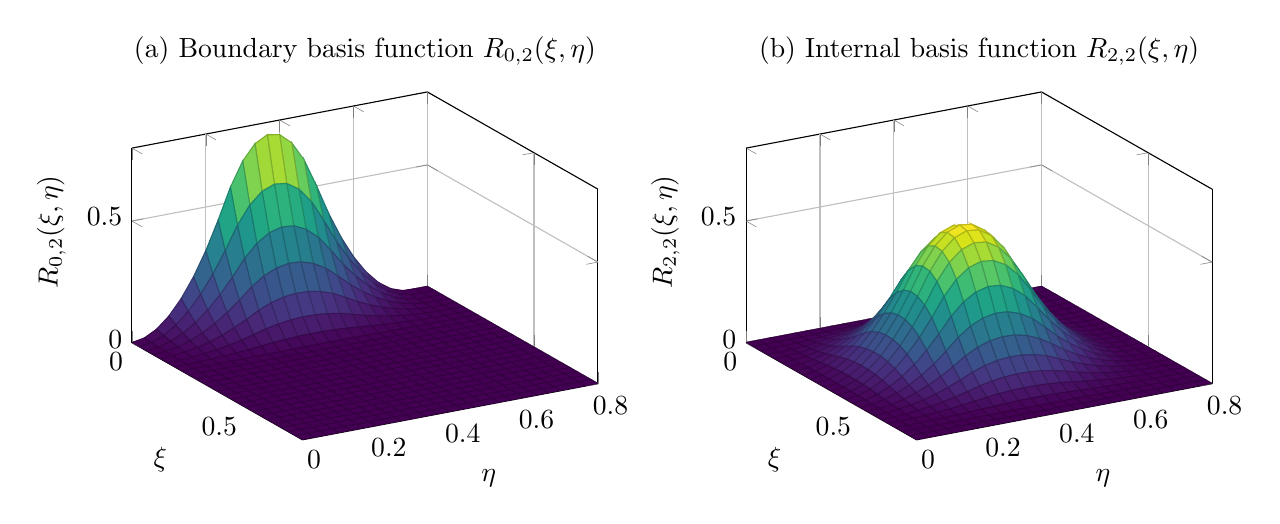
\begin{tikzpicture}[
                declare function={
                        n0(\t) = (\t < 0.25) * ((1-4*\t)^2);
                        n2(\t) = (\t < 0.25) * (8*\t^2) +
                        (\t >= 0.25) * (\t < 0.5) * (12*\t - 16*\t^2 - 1.5) +
                        (\t >= 0.5) * (\t < 0.75) * (8*(0.75-\t)^2);
                    }
            ]
            % Panel (a) Axis
            \begin{axis}[
                    at={(0,0)},
                    width=7.5cm,
                    height=6.0cm,
                    grid=major,
                    xlabel={$\xi$},
                    ylabel={$\eta$},
                    zlabel={$R_{0,2}(\xi,\eta)$},
                    colormap/viridis,
                    view={60}{30},
                    zmin=0, zmax=0.8,
                    title={(a) Boundary basis function $R_{0,2}(\xi,\eta)$}
                ]
                \addplot3[
                    surf,
                    domain=0:0.8,
                    domain y=0:0.8,
                    samples=25,
                    shader=faceted
                ] {n0(x)*n2(y)};
            \end{axis}

            % Panel (b) Axis
            \begin{axis}[
                    at={(7.8cm,0)},
                    width=7.5cm,
                    height=6.0cm,
                    grid=major,
                    xlabel={$\xi$},
                    ylabel={$\eta$},
                    zlabel={$R_{2,2}(\xi,\eta)$},
                    colormap/viridis,
                    view={60}{30},
                    zmin=0, zmax=0.8,
                    title={(b) Internal basis function $R_{2,2}(\xi,\eta)$}
                ]
                \addplot3[
                    surf,
                    domain=0:0.8,
                    domain y=0:0.8,
                    samples=25,
                    shader=faceted
                ] {n2(x)*n2(y)};
            \end{axis}
        \end{tikzpicture}%
    }
    \caption{3D surface plots of two distinct bivariate tensor-product B-spline basis functions: (a) boundary basis function $R_{0,2}(\xi,\eta) = N_{0,2}(\xi)M_{2,2}(\eta)$ and (b) internal basis function $R_{2,2}(\xi,\eta) = N_{2,2}(\xi)M_{2,2}(\eta)$, demonstrating edge-supported versus fully internal support.}
    \label{fig:bivariate_basis_3d}
\end{figure}

The physical domain surface $\vect{S}(\xi, \eta)$ is constructed as a linear combination of a 2D control point lattice $\vect{P}_{i,j}$, as shown in Figure \ref{fig:bspline_surface_concept}:
\begin{equation}
    \vect{S}(\xi, \eta) = \sum_{i=0}^{n-1} \sum_{j=0}^{m-1} R_{i,j}^{p,q}(\xi, \eta) \vect{P}_{i,j}
\end{equation}

For surface integration, parametric gradients map to physical space via 2D coordinate Jacobian $\mat{J}$:
\begin{equation}
    \mat{J}(\xi, \eta) = \begin{bmatrix} \frac{\partial x}{\partial \xi} & \frac{\partial y}{\partial \xi} \\[0.3em] \frac{\partial x}{\partial \eta} & \frac{\partial y}{\partial \eta} \end{bmatrix} = \begin{bmatrix} \sum \frac{\partial R_{i,j}^{p,q}}{\partial \xi} x_{i,j} & \sum \frac{\partial R_{i,j}^{p,q}}{\partial \xi} y_{i,j} \\[0.5em] \sum \frac{\partial R_{i,j}^{p,q}}{\partial \eta} x_{i,j} & \sum \frac{\partial R_{i,j}^{p,q}}{\partial \eta} y_{i,j} \end{bmatrix}
\end{equation}
The local outward unit surface normal vector $\vect{n}(\xi, \eta)$ is extracted via the cross product:
\begin{equation}
    \vect{n}(\xi, \eta) = \frac{\vect{g}_{\xi} \times \vect{g}_{\eta}}{\|\vect{g}_{\xi} \times \vect{g}_{\eta}\|}
\end{equation}
where $\vect{g}_{\xi} = \partial \vect{S}/\partial \xi$ and $\vect{g}_{\eta} = \partial \vect{S}/\partial \eta$.

\begin{figure}[htbp]
    \centering
    \begin{tikzpicture}[scale=1.0, >=stealth]
        \coordinate (P00) at (0, 0);   \coordinate (P10) at (2, 0.2);   \coordinate (P20) at (4, 0);
        \coordinate (P01) at (0.5, 1.0); \coordinate (P11) at (2.5, 1.7); \coordinate (P21) at (4.5, 1.0);
        \coordinate (P02) at (1.0, 2.0); \coordinate (P12) at (3.0, 2.2); \coordinate (P22) at (5.0, 2.0);

        \draw[thick, gray!60, dashed] (P00) -- (P10) -- (P20);
        \draw[thick, gray!60, dashed] (P01) -- (P11) -- (P21);
        \draw[thick, gray!60, dashed] (P02) -- (P12) -- (P22);
        \draw[thick, gray!60, dashed] (P00) -- (P01) -- (P02);
        \draw[thick, gray!60, dashed] (P10) -- (P11) -- (P12);
        \draw[thick, gray!60, dashed] (P20) -- (P21) -- (P22);

        \fill[lightbg, opacity=0.8, draw=primaryblue, thick]
        (P00) .. controls (1.0, 0.1) and (3.0, 0.1) .. (P20)
        .. controls (4.3, 0.6) and (4.7, 1.4) .. (P22)
        .. controls (4.0, 2.1) and (2.0, 2.1) .. (P02)
        .. controls (0.7, 1.4) and (0.3, 0.6) .. (P00);

        \draw[primaryblue!40, thin] (1.0, 0.1) .. controls (1.5, 1.0) and (2.0, 1.7) .. (2.0, 2.1);
        \draw[primaryblue!40, thin] (3.0, 0.1) .. controls (3.2, 1.0) and (3.5, 1.7) .. (4.0, 2.1);
        \draw[primaryblue!40, thin] (0.5, 1.0) .. controls (1.5, 1.3) and (3.5, 1.3) .. (4.5, 1.0);

        \foreach \p in {P00, P01, P02, P10, P11, P12, P20, P21, P22} {
                \fill[red!80!black] (\p) circle (2.5pt);
            }

        \node[red!80!black, above, fill=white, inner sep=1pt] at (P11) {$\vect{P}_{i,j}$};
        \node[primaryblue] at (2.5, 1.0) {\textbf{$\vect{S}(\xi,\eta)$}};
    \end{tikzpicture}
    \caption{Bivariate B-spline surface patch $\vect{S}(\xi,\eta)$ guided by a control lattice $\vect{P}_{i,j}$.}
    \label{fig:bspline_surface_concept}
\end{figure}

By linking parametric coordinates to a 3D control lattice $\vect{P}_{i,j}$ (Figure \ref{fig:bspline_surface_concept}), bivariate NURBS patches construct exact geometric surfaces $\vect{S}(\xi, \eta)$.

% ------------------------------------------------------------------------------
\section{\texorpdfstring{Refinement Strategies: $h$-, $p$-, \& $k$-Refinement}{Refinement Strategies}}
% ------------------------------------------------------------------------------

The following discussion details the three refinement mechanisms of IGA that enable mesh enrichment without altering the exact CAD geometry.

A major advantage of IGA is mesh refinement without modifying CAD geometry definitions:

\begin{table}[htbp]
    \centering
    \caption{Comparative synthesis of IGA refinement mechanisms.}
    \label{tab:refinement_comparison}
    \resizebox{\textwidth}{!}{%
        \begin{tabular}{l l l l p{5.5cm}}
            \toprule
            \textbf{Refinement Type} & \textbf{Mechanism} & \textbf{Continuity}  & \textbf{Exact CAD Geometry} & \textbf{Primary Advantage / Impact}                              \\
            \midrule
            \textbf{$h$-Refinement}  & Knot Insertion     & Retained ($C^{p-1}$) & Preserved Exactly           & Local mesh enrichment near stress concentrations (notches).      \\
            \textbf{$p$-Refinement}  & Degree Elevation   & Increased ($C^p$)    & Preserved Exactly           & Higher-order accuracy without Runge oscillatory phenomena.       \\
            \textbf{$k$-Refinement}  & Order Elevation    & Maximum ($C^{p-1}$)  & Preserved Exactly           & Superior accuracy per DOF; non-local basis with high continuity. \\
            \bottomrule
        \end{tabular}%
    }
\end{table}

Comparing these three refinement pathways (Table \ref{tab:refinement_comparison}) shows that IGA enables arbitrary mesh enrichment while maintaining strict $C^{p-1}$ continuity and exact CAD boundary definitions.

\subsection{Boehm Knot Insertion Algorithm (\texorpdfstring{$h$-Refinement}{h-Refinement})}
Boehm's algorithm for knot insertion ($h$-refinement) enables local mesh refinement near stress concentrations.

In $h$-refinement, new control points $\vect{P}_i^{\text{new}}$ are computed via Boehm's algorithm:
\begin{equation}
    \vect{P}_i^{\text{new}} = \alpha_i \vect{P}_i + (1 - \alpha_i) \vect{P}_{i-1}
\end{equation}
where blending coefficients $\alpha_i$ are:
\begin{equation}
    \alpha_i = \begin{cases}
        1                                           & \text{if } i \le k - p           \\
        \frac{\bar{\xi} - \xi_i}{\xi_{i+p} - \xi_i} & \text{if } k - p + 1 \le i \le k \\
        0                                           & \text{if } i \ge k + 1
    \end{cases}
\end{equation}

For 2D domains with lattice matrix $\mat{P}$, directional transformations $\mat{T}_{\xi}$ and $\mat{T}_{\eta}$ yield:
\begin{equation}
    \mat{P}^{\text{new}} = \mat{T}_{\xi} \mat{P} \mat{T}_{\eta}^T, \quad \vect{P}^{\text{new}} = \left( \mat{T}_{\eta} \otimes \mat{T}_{\xi} \right) \vect{P}
\end{equation}

Degree elevation ($p$-refinement) operates via $\vect{P}^{\text{new}} = \mat{T}_p \vect{P}$.

Demonstrating $h$-refinement (knot insertion) confirms how the control polygon refines while preserving exact curve geometry (Figure \ref{fig:hrefinement_basis}).

\begin{figure}[htbp]
    \centering
    \makebox[\textwidth][c]{%
        \begin{tikzpicture}[scale=0.9, >=stealth]
            % Row 1: Basis functions before/after
            \begin{scope}[yshift=3.6cm]
                \draw[->, thick, black!70] (0,0) -- (4.2,0) node[right] {$\xi$};
                \draw[->, thick, black!70] (0,0) -- (0,2.2) node[above] {$N_{i,2}$};
                \draw[gray!30, thin] (0,0) grid[ystep=0.5, xstep=1.0] (4,2);
                \draw[blue, line width=1.2pt, domain=0:4] plot (\x, {2*(1 - \x/4)^2});
                \draw[green!60!black, line width=1.2pt, domain=0:4] plot (\x, {2*2*(\x/4)*(1 - \x/4)});
                \draw[orange, line width=1.2pt, domain=0:4] plot (\x, {2*(\x/4)^2});
                \node[font=\tiny, below] at (2, -0.1) {$\Xi = \{0,0,0,1,1,1\}$};
            \end{scope}
            \begin{scope}[xshift=5.0cm, yshift=3.6cm]
                \draw[->, thick, black!70] (0,0) -- (4.2,0) node[right] {$\xi$};
                \draw[->, thick, black!70] (0,0) -- (0,2.2) node[above] {$N_{i,2}$};
                \draw[gray!30, thin] (0,0) grid[ystep=0.5, xstep=1.0] (4,2);
                \draw[blue, line width=1.2pt, domain=0:2] plot (\x, {2*(1 - \x/2)^2});
                \draw[green!60!black, line width=1.2pt, domain=0:2] plot (\x, {2*(4*(\x/4) - 6*(\x/4)^2)});
                \draw[green!60!black, line width=1.2pt, domain=2:4] plot (\x, {2*(2*(1-\x/4)^2)});
                \draw[orange, line width=1.2pt, domain=0:2] plot (\x, {2*(2*(\x/4)^2)});
                \draw[orange, line width=1.2pt, domain=2:4] plot (\x, {2*(4*(1-\x/4) - 6*(1-\x/4)^2)});
                \draw[red, line width=1.2pt, domain=2:4] plot (\x, {2*((\x-2)/2)^2});
                \node[font=\tiny, below] at (2, -0.1) {$\Xi = \{0,0,0,0.5,1,1,1\}$};
            \end{scope}

            % Row 2: Curves and control polygons before/after
            \begin{scope}[xshift=0cm, yshift=0cm]
                \draw[gray!20, thin] (0,0) grid (3.6,2.5);
                \draw[gray!70, dashed, line width=0.8pt] (0,0) -- (1.8,2.2) -- (3.6,0);
                \fill[red!80!black] (0,0) circle (2pt);
                \fill[red!80!black] (1.8,2.2) circle (2pt);
                \fill[red!80!black] (3.6,0) circle (2pt);
                \draw[primaryblue, line width=1.5pt, domain=0:1] plot ({3.6*\x}, {4.4*\x*(1-\x)});
                \node[primaryblue, above, font=\scriptsize] at (1.8, 1.2) {$\vect{C}(\xi)$};
                \node[font=\tiny, below] at (1.8, -0.1) {Original polygon \& curve};
            \end{scope}
            \begin{scope}[xshift=5.0cm, yshift=0cm]
                \draw[gray!20, thin] (0,0) grid (3.6,2.5);
                \draw[gray!70, dashed, line width=0.8pt] (0,0) -- (0.9,1.1) -- (2.7,1.1) -- (3.6,0);
                \fill[red!80!black] (0,0) circle (2pt);
                \fill[red!80!black] (0.9,1.1) circle (2pt);
                \fill[red!80!black] (2.7,1.1) circle (2pt);
                \fill[red!80!black] (3.6,0) circle (2pt);
                \draw[primaryblue, line width=1.5pt, domain=0:1] plot ({3.6*\x}, {4.4*\x*(1-\x)});
                \node[primaryblue, above, font=\scriptsize] at (1.8, 1.2) {$\vect{C}(\xi)$};
                \node[font=\tiny, below] at (1.8, -0.1) {Refined polygon (knot inserted)};
            \end{scope}
        \end{tikzpicture}%
    }
    \caption{$h$-refinement (knot insertion) schema showing basis functions before/after inserting knot $\xi=0.5$ (top) and corresponding control polygon refinement while preserving exact curve geometry (bottom).}
    \label{fig:hrefinement_basis}
\end{figure}

Inserting knots via Boehm's algorithm (Figure \ref{fig:hrefinement_basis}) enriches the control polygon density while preserving the exact CAD geometry.

\subsection{Degree Elevation (\texorpdfstring{$p$-Refinement}{p-Refinement})}
Degree elevation ($p$-refinement) increases the polynomial order $p$ of the NURBS basis functions without modifying the underlying CAD geometry or introducing new knot spans.

Starting from a curve of polynomial degree $p$ defined over knot vector $\Xi = \{\xi_0, \xi_1, \dots, \xi_m\}$, degree elevation increases the polynomial order from $p$ to $p+t$. To preserve the original continuity $C^{p-m_i}$ at each distinct knot $\xi_i$ with original multiplicity $m_i$, the multiplicity of each knot in the elevated knot vector $\Xi^{\text{new}}$ is increased to $m_i + t$.

The updated control points $\vect{P}_i^{\text{new}}$ are computed via a degree elevation transformation matrix $\mat{T}_p$:
\begin{equation}
    \vect{P}^{\text{new}} = \mat{T}_p \vect{P}
\end{equation}

Unlike classical finite element $p$-refinement, IGA degree elevation retains higher-order inter-element continuity ($C^{p+t-m_i}$) across knot spans while completely eliminating Runge oscillatory phenomena (Figure \ref{fig:prefinement_basis}).

\begin{figure}[htbp]
    \centering
    \makebox[\textwidth][c]{%
        \begin{tikzpicture}[scale=0.9, >=stealth]
            % Row 1: Basis functions before/after
            \begin{scope}[yshift=3.6cm]
                \draw[->, thick, black!70] (0,0) -- (4.2,0) node[right] {$\xi$};
                \draw[->, thick, black!70] (0,0) -- (0,2.2) node[above] {$N_{i,1}$};
                \draw[gray!30, thin] (0,0) grid[ystep=0.5, xstep=1.0] (4,2);
                \draw[blue, line width=1.2pt] (0,2) -- (4,0);
                \draw[green!60!black, line width=1.2pt] (0,0) -- (4,2);
                \node[font=\tiny, below] at (2, -0.1) {$p=1$, $\Xi = \{0,0,1,1\}$};
            \end{scope}
            \begin{scope}[xshift=5.0cm, yshift=3.6cm]
                \draw[->, thick, black!70] (0,0) -- (4.2,0) node[right] {$\xi$};
                \draw[->, thick, black!70] (0,0) -- (0,2.2) node[above] {$N_{i,2}$};
                \draw[gray!30, thin] (0,0) grid[ystep=0.5, xstep=1.0] (4,2);
                \draw[blue, line width=1.2pt, domain=0:4] plot (\x, {2*(1 - \x/4)^2});
                \draw[green!60!black, line width=1.2pt, domain=0:4] plot (\x, {2*2*(\x/4)*(1 - \x/4)});
                \draw[orange, line width=1.2pt, domain=0:4] plot (\x, {2*(\x/4)^2});
                \node[font=\tiny, below] at (2, -0.1) {$p=2$, $\Xi = \{0,0,0,1,1,1\}$};
            \end{scope}

            % Row 2: Curves and control polygons before/after
            \begin{scope}[xshift=0cm, yshift=0cm]
                \draw[gray!20, thin] (0,0) grid (3.6,2.5);
                \draw[gray!70, dashed, line width=0.8pt] (0,0) -- (1.8,2.2) -- (3.6,0);
                \fill[red!80!black] (0,0) circle (2pt);
                \fill[red!80!black] (1.8,2.2) circle (2pt);
                \fill[red!80!black] (3.6,0) circle (2pt);
                \draw[primaryblue, line width=1.5pt, domain=0:1] plot ({3.6*\x}, {4.4*\x*(1-\x)});
                \node[primaryblue, above, font=\scriptsize] at (1.8, 1.2) {$\vect{C}(\xi)$};
                \node[font=\tiny, below] at (1.8, -0.1) {Original curve ($p=2$)};
            \end{scope}
            \begin{scope}[xshift=5.0cm, yshift=0cm]
                \draw[gray!20, thin] (0,0) grid (3.6,2.5);
                \draw[gray!70, dashed, line width=0.8pt] (0,0) -- (1.2,1.5) -- (2.4,1.5) -- (3.6,0);
                \fill[red!80!black] (0,0) circle (2pt);
                \fill[red!80!black] (1.2,1.5) circle (2pt);
                \fill[red!80!black] (2.4,1.5) circle (2pt);
                \fill[red!80!black] (3.6,0) circle (2pt);
                \draw[primaryblue, line width=1.5pt, domain=0:1] plot ({3.6*\x}, {4.4*\x*(1-\x)});
                \node[primaryblue, above, font=\scriptsize] at (1.8, 1.2) {$\vect{C}(\xi)$};
                \node[font=\tiny, below] at (1.8, -0.1) {Degree elevated ($p=3$)};
            \end{scope}
        \end{tikzpicture}%
    }
    \caption{$p$-refinement (degree elevation) schema showing basis functions (top) and B-spline curves (bottom) before/after elevating polynomial degree from $p=1$ to $p=2$.}
    \label{fig:prefinement_basis}
\end{figure}

\subsection{Order Elevation (\texorpdfstring{$k$-Refinement}{k-Refinement})}
Unique to Isogeometric Analysis, $k$-refinement commutes degree elevation and knot insertion to construct high-order basis functions with maximum inter-element continuity ($C^{p-1}$).

In traditional finite element analysis (or standard $p$-refinement applied after mesh subdivision), knot insertion followed by degree elevation results in $C^0$ continuity across element boundaries. In contrast, $k$-refinement executes these operations in reverse order:
\begin{enumerate}[leftmargin=*]
    \item \textbf{Degree Elevation First}: The polynomial degree of the coarse curve or surface patch is elevated from $p$ to $p+t$, raising internal continuity to $C^{p+t-1}$.
    \item \textbf{Knot Insertion Second}: Knots are subsequently inserted into the elevated knot vector, retaining the maximum achievable inter-element continuity $C^{p+t-1}$ across all newly created knot spans.
\end{enumerate}

By maintaining maximum inter-element continuity, $k$-refinement significantly reduces the total number of active control variables (degrees of freedom) required per element compared to standard $p$-FEM, offering superior spectral accuracy per degree of freedom for dynamic structural simulations (Figure \ref{fig:krefinement_basis}).

\begin{figure}[htbp]
    \centering
    \makebox[\textwidth][c]{%
        \begin{tikzpicture}[scale=1.05, >=stealth]
            % --- PANEL (a) BEFORE ---
            \begin{scope}[xshift=0cm]
                \draw[gray!15, thin, step=0.5] (-1.4, -1.4) grid (1.4, 1.4);
                \draw[->, black!40, line width=0.5pt] (-1.5, 0) -- (1.5, 0);
                \draw[->, black!40, line width=0.5pt] (0, -1.5) -- (0, 1.5);
                \draw[primaryblue, thick] (0,0) circle (1.0);
                \draw[gray!70, dashed, thick] (1,0) -- (1,1) -- (0,1) -- (-1,1) -- (-1,0) -- (-1,-1) -- (0,-1) -- (1,-1) -- cycle;
                \foreach \x/\y in {1/0, 0/1, -1/0, 0/-1, 1/1, -1/1, -1/-1, 1/-1} {
                        \fill[red!80!black] (\x, \y) circle (2.2pt);
                    }
                \node[font=\tiny, fill=white, inner sep=1pt, draw=gray!20] at (1.2, 0.4) {$w_{\text{diag}}\approx 0.707$};
                \node[below=1.5cm, font=\scriptsize\bfseries] at (0,0) {(a) Initial Geometry (8 Control Points)};
            \end{scope}

            % --- PANEL (b) AFTER ---
            \begin{scope}[xshift=6.1cm]
                \draw[gray!15, thin, step=0.5] (-1.4, -1.4) grid (1.4, 1.4);
                \draw[->, black!40, line width=0.5pt] (-1.5, 0) -- (1.5, 0);
                \draw[->, black!40, line width=0.5pt] (0, -1.5) -- (0, 1.5);
                \draw[primaryblue, thick] (0,0) circle (1.0);
                \draw[gray!70, dashed, thick] (0:1.025)
                \foreach \angle in {22.5, 45, 67.5, 90, 112.5, 135, 157.5, 180, 202.5, 225, 247.5, 270, 292.5, 315, 337.5, 360} {
                        -- (\angle:1.025)
                    };
                \foreach \angle in {0, 22.5, 45, 67.5, 90, 112.5, 135, 157.5, 180, 202.5, 225, 247.5, 270, 292.5, 315, 337.5} {
                        \fill[red!80!black] (\angle:1.025) circle (2.2pt);
                    }
                \node[below=1.5cm, font=\scriptsize\bfseries] at (0,0) {(b) After $k$-Refinement (16 Control Points)};
            \end{scope}
        \end{tikzpicture}%
    }
    \caption{$k$-refinement (order elevation) schema demonstrating exact circle CAD geometry preservation with increased control point density and maximum inter-element continuity $C^{p-1}$.}
    \label{fig:krefinement_basis}
\end{figure}
\newpage
% ------------------------------------------------------------------------------
\section{Isogeometric System Matrix Assembly}
% ------------------------------------------------------------------------------

Here, we detail the Galerkin projection of elastodynamic fields onto NURBS basis functions to assemble global mass $\mat{M}$, stiffness $\mat{K}$, and force $\vect{F}_{\text{ext}}$ matrices.

Approximating the displacement field using bivariate NURBS basis functions $R_a(\vect{x})$ yields:
\begin{equation}
    \vect{u}_h(\vect{x}, t) = \sum_{a=1}^{n_b} R_a(\vect{x}) \vect{d}_a(t)
\end{equation}
where explicit analytical derivatives $\frac{\partial R_a}{\partial \xi}$ and $\frac{\partial R_a}{\partial \eta}$ required for strain matrix assembly are detailed in Appendix \ref{sec:appendix_nurbs_derivatives}, and $\vect{d}_a(t) \in \mathbb{R}^2$ represents control variable displacements. Substituting into the weak form leads to the semi-discrete equations of motion:

\begin{equation}
    \mathbf{M}\ddot{\vect{d}}(t) + \mathbf{C}\dot{\vect{d}}(t) + \mathbf{K}\vect{d}(t) = \vect{F}_{\text{ext}}(t)
\end{equation}

where global matrices are assembled from element integrals over knot spans $\Omega_e$:
\begin{align}
    \mathbf{M}_{ab}   & = \int_{\Omega_e} \rho R_a R_b \mathbf{I}_2 \, d\Omega                                      \\
    \mathbf{K}_{ab}   & = \int_{\Omega_e} \mathbf{B}_a^T \mathbf{D} \mathbf{B}_b \, d\Omega                         \\
    \vect{F}_{ext, a} & = \int_{\Omega_e} R_a \vect{f}_b \, d\Omega + \int_{\Gamma_{N,e}} R_a \vect{h}_N \, d\Gamma
\end{align}

Here, $\mathbf{B}_a$ represents the strain-displacement matrix containing parametric derivatives of $R_a(\vect{x})$ mapped via the spatial Jacobian $\mathbf{J}(\xi, \eta)$.

To justify selecting the $80 \times 40$ element baseline for the full-order model, we perform a grid convergence study under static bending and validate accuracy against classical Lagrangian Finite Element methods.

% ------------------------------------------------------------------------------
\section{Mesh Convergence \& Accuracy Validation}
% ------------------------------------------------------------------------------

Here, we state the physical load conditions, plane stress assumptions, and numerical setup governing the mesh convergence study, followed by accuracy benchmarks against Lagrangian FEM.

\subsection{Simulation Conditions \& Boundary Assumptions}
The mesh convergence study models a notched cantilever beam of length $L = 2.0\text{ m}$ and height $H = 0.4\text{ m}$ subjected to a static vertical tip load $F_y = -10\text{ kN}$ applied at the free right boundary ($\xi = 1$). The fixed root boundary at $\xi = 0$ is fully clamped ($\vect{u} = \mathbf{0}$).

The material is assumed homogeneous, isotropic, and linearly elastic with Young's modulus $E = 210\text{ GPa}$, Poisson's ratio $\nu = 0.3$, and mass density $\rho = 7850\text{ kg/m}^3$. Under plane stress conditions, the constitutive tensor $\mat{D}$ is given by:
\begin{equation}
    \mat{D} = \frac{E}{1 - \nu^2} \begin{bmatrix} 1 & \nu & 0 \\ \nu & 1 & 0 \\ 0 & 0 & \frac{1 - \nu}{2} \end{bmatrix}
\end{equation}

Analytical spatial strain-displacement matrices $\mathbf{B}_a$ map nodal shape function gradients using the parametric Jacobian $\mat{J}(\xi, \eta)$.

\subsection{Grid Convergence Analysis via \texorpdfstring{$k$-Refinement}{k-Refinement}}
To construct a convergent mesh while maximizing accuracy per degree of freedom, the convergence study employs $k$-refinement as implemented in the web-based simulation visualizer (\texttt{iga-sim-5.3}):
\begin{enumerate}[leftmargin=*]
    \item \textbf{Degree Elevation First}: The initial coarse CAD patch is elevated to quadratic degree ($p=2, q=2$), establishing $C^1$ continuity across the parametric domain.
    \item \textbf{Knot Insertion Second}: Dyadic knot insertion is subsequently performed on the elevated patch, refining the mesh resolution from $10 \times 5$ ($50$ elements, $168$ DOFs) up to a fine reference grid of $160 \times 80$ ($12,800$ elements, $26,568$ DOFs).
\end{enumerate}

Because degree elevation precedes knot insertion, all inserted internal knot spans preserve maximum $C^{p-1} = C^1$ inter-element continuity. Vertical tip displacement $U_y$ and relative error evaluated against the $160 \times 80$ fine reference solution ($U_y = 4.238\text{ mm}$) are summarized in Table \ref{tab:mesh_convergence}.

\begin{table}[htbp]
    \centering
    \caption{Mesh convergence study for the notched cantilever beam under static bending load using $k$-refinement ($p=2, C^1$ continuity), evaluating vertical tip displacement $U_y$ and relative error across dyadic resolutions.}
    \label{tab:mesh_convergence}
    \begin{tabular}{lcccc}
        \toprule
        \textbf{Resolution}     & \textbf{Elements} & \textbf{DoFs}  & \textbf{Tip Disp. $U_y$ (mm)} & \textbf{Relative Error (\%)} \\
        \midrule
        $10 \times 5$           & $50$              & $168$          & $3.538$                       & $16.51\%$                    \\
        $20 \times 10$          & $200$             & $528$          & $3.889$                       & $8.24\%$                     \\
        $40 \times 20$          & $800$             & $1,848$        & $4.083$                       & $3.66\%$                     \\
        \textbf{80 $\times$ 40} & \textbf{3,200}    & \textbf{6,888} & \textbf{4.185}                & \textbf{1.24\%}              \\
        $160 \times 80$         & $12,800$          & $26,568$       & $4.238$                       & Reference                    \\
        \bottomrule
    \end{tabular}
\end{table}

Refining from $80 \times 40$ ($3,200$ elements) to $160 \times 80$ ($12,800$ elements) yields only a $1.24\%$ shift in tip displacement while increasing equations by $3.8\times$, confirming $80 \times 40$ ($6,888$ DOFs) as an optimal, convergent baseline for full-order elastodynamic simulations.

\subsection{Linear Accuracy Validation Against Lagrangian FEM}
To assess the accuracy and efficiency of the bivariate NURBS discretization compared to classical $C^0$ Lagrangian Finite Element methods, the full-order IGA baseline ($80 \times 40$ elements) is benchmarked against a fine-mesh Lagrangian FEM model ($12,400$ DOFs). The validation metrics are reported in Table \ref{tab:linear_validation}.

\begin{table}[htbp]
    \centering
    \caption{Linear solution accuracy validation comparing full-order IGA degrees of freedom against fine-mesh Lagrangian FEM frameworks.}
    \label{tab:linear_validation}
    \resizebox{\textwidth}{!}{%
        \begin{tabular}{lcccc}
            \toprule
            \textbf{Mesh Setup} & \textbf{Total DoFs} & \textbf{Tip Disp. (mm)} & \textbf{Energy Norm (J)}     & \textbf{Solve Time (ms)} \\
            \midrule
            Lagrangian FEM      & $12,400$            & $4.182$                 & $1.042 \times 10^5$          & $845.2$                  \\
            \textbf{IGA Core}   & \textbf{6,888}      & \textbf{4.185}          & \textbf{1.044 $\times 10^5$} & \textbf{142.1}           \\
            \bottomrule
        \end{tabular}%
    }
\end{table}

Owing to the inter-element $C^{p-1}$ continuity of quadratic NURBS basis functions, the IGA core achieves equivalent tip displacement accuracy ($4.185\text{ mm}$ vs. $4.182\text{ mm}$) with $44\%$ fewer DOFs and a $6\times$ reduction in linear solver computation time ($142.1\text{ ms}$ vs. $845.2\text{ ms}$).

% ------------------------------------------------------------------------------
\section{Chapter Summary}
% ------------------------------------------------------------------------------

In closing, we summarize the IGA discretization framework and establish the transition to Chapter \ref{ch:pullback} for reference domain pullback mapping.

\begin{tcolorbox}[colback=lightbg, colframe=accentcyan, title=\textbf{Key Takeaway}, fonttitle=\bfseries]
    Isogeometric Analysis discretizes the continuous elastodynamic equations using exact NURBS CAD geometry basis functions, assembling the full-order matrices $\mathbf{M}$, $\mathbf{K}$, and $\mathbf{C}$. In Chapter \ref{ch:pullback}, we pull back these element integrals to a parameter-independent reference configuration $\hat{\Omega}$ to resolve shape parameter compatibility.
\end{tcolorbox}
